
In this section we will dive a bit deeper and analyze the results we collected in the previous section and present the data in diagrams to ease the comparisons. 


\vspace{0.5cm}
\subsection{Hardware and Time Complexity}
\label{sec:4.1}
In order to be able to answer our initial question we wanted to make sure whether or not hardware have any impact on the overall difference between the three time complexities the algorithms we are working with represent.  

\begin{figure}[H]
  \makebox[\textwidth][c]{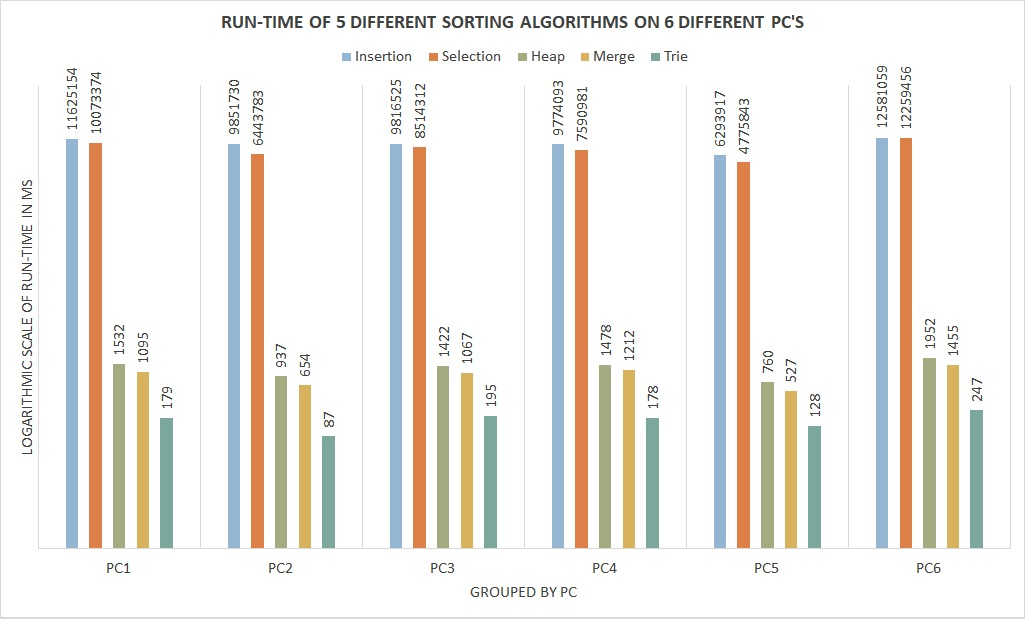
\includegraphics[width=1.2\textwidth]{figures/runtime1.jpg}}
  \caption{Logarithmic scale representation of the algorithms run-runtime on the six PCs.}
  \label{fig:pic1}
\end{figure}
In figure~\ref{fig:pic1} above, which is made from the data presented in table~\ref{tab:timings1} on page~\pageref{tab:timings1} it is clear to see both the run-time of each sorting algorithm and the apparent jumps between the time complexity for all the PCs. 

\vspace{0.5cm}
\subsection{Measurements on varying data amounts}
\label{sec:4.2}
As mentioned we decided to run all algorithms on the same PC with varying amounts of data to be able to make more direct comparisons between the five algorithms. The data used to create the following diagrams can be seen in table~\ref{tab:PC2timings} on page~\pageref{tab:PC2timings}. 
\begin{figure}[H]
  \makebox[\textwidth][c]{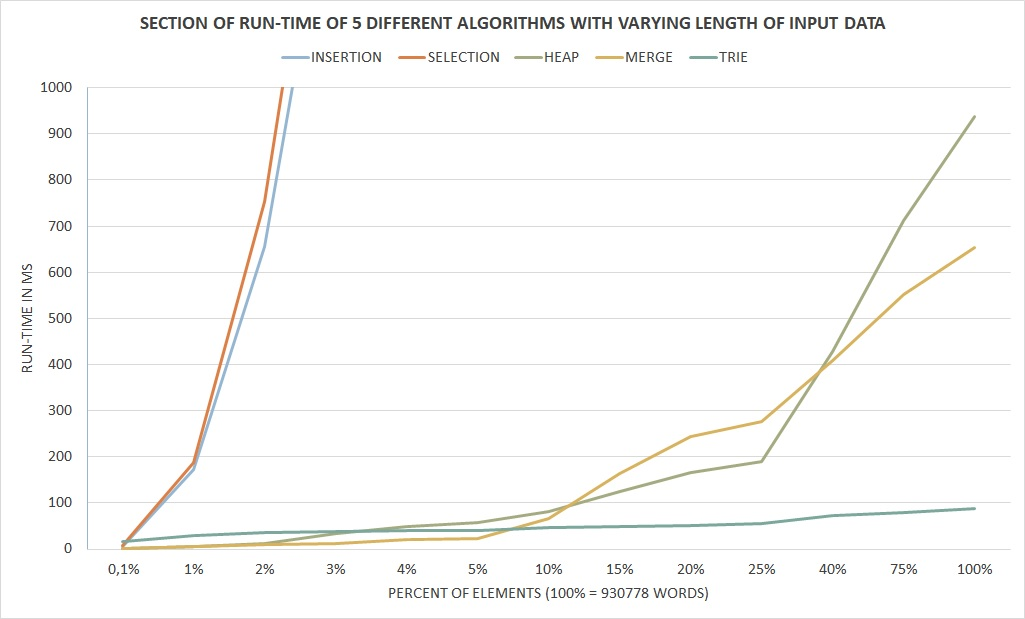
\includegraphics[width=1.1\textwidth]{figures/runtime2.jpg}}
  \caption{Timings ranging from 2ms to 1000ms. 100\% equals 930778 words}
  \label{fig:pic2}
\end{figure}

\begin{figure}[H]
  \makebox[\textwidth][c]{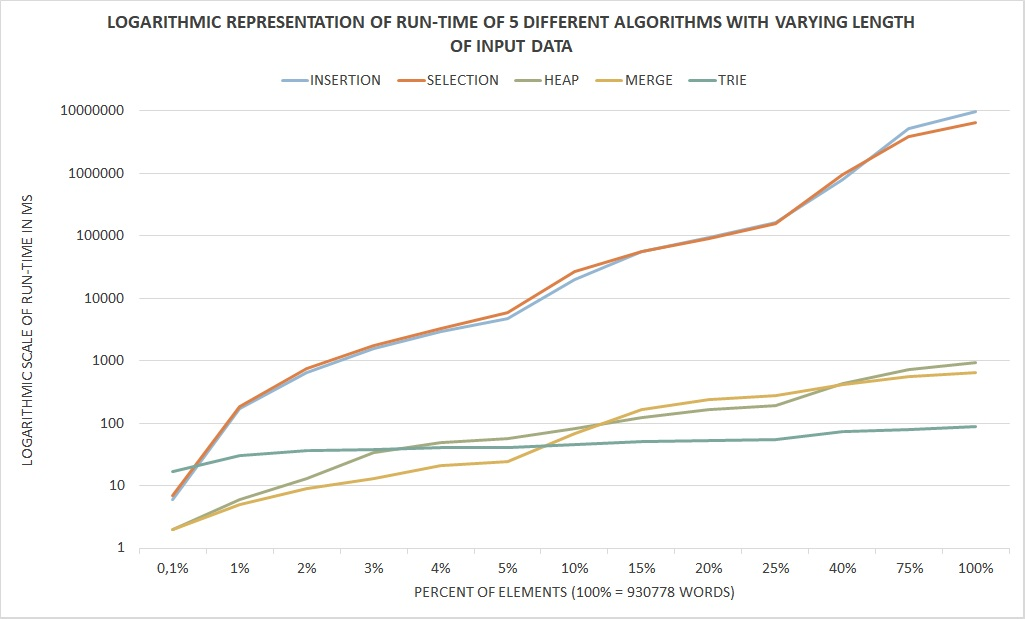
\includegraphics[width=1.1\textwidth]{figures/runtime3.jpg}}
  \caption{All timings represented on a logarithmic scale. 100\% equals 930778 words}
  \label{fig:pic3}
\end{figure}

Figure~\ref{fig:pic2} shows a smaller section of the timings in order to be able to see all the sorting algorithm graphs clearly, with the varying data amounts. This representation of the data is useful for an overall view of the differences, but in order to compare further we need to look at a logarithmic diagram. 
\\
Figure~\ref{fig:pic3} shows all of the timing data on a logarithmic scale with the varying data amounts. On a graph represented on a logarithmic scale, as in figure~\ref{fig:pic3}, the distinction between the efficiency for small amounts of data become more clear.







